%-----------------------------------------------------------------------------------------------
\section{Reversible Stirling Engine Model}

    In     this     section,     Cheng     and     Yang's     reversible     Stirling     engine
    model~\cite{2012-ChengCH+YangHS-ApEnergy} is presented. Owing to the context in  which  such
    example is regarded useful, only a concise subset of the model that is useful for the stated
    goal of the present work is being presented, as to avoid unnecessary distractions.

    Moreover, the model nomenclature  is  kept  the  same  as  the  one  used  in  the  original
    reference~\cite{2012-ChengCH+YangHS-ApEnergy}, so as to allow readers to  easily  lookup  in
    the original work the parts abridged in  this  work.  There  is  only  a  minute  change  in
    nomenclature employed herein for conciseness, which consists in annotating the greek  letter
    of the engine configuration above a symbol, so as to specify that  symbol's  expression  for
    that particular engine configuration, starting on Eq.~(\ref{eq:Ve}).

    \begin{figure}[ht]
        \centering
        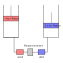
\includegraphics[width=0.7\columnwidth]{fig/stirling_engine_alpha_color.pdf}
        \caption{Schematic representation of an ideal Stirling engine of the $\alpha$-type.  The
            `eHX'  and  the  `cHX'  are  the  `expansion'  and  `compression'  heat  exchangers,
            respectively of high- and low- temperatures. The power pistons and  the  regenerator
            are indicated. Volumes are not to scale.}
        \label{fig:alpha}
    \end{figure}

    \begin{figure}[ht]
        \centering
        \includegraphics[width=0.7\columnwidth]{fig/stirling_engine_beta_color.pdf}
        \caption{Schematic representation of an ideal Stirling engine of the  $\beta$-type.  The
            `eHX'  and  the  `cHX'  are  the  `expansion'  and  `compression'  heat  exchangers,
            respectively of high- and low- temperatures. The power and displacement pistons  and
            the regenerator are indicated. Volumes are not to scale.}
        \label{fig:beta}
    \end{figure}

    Let $V_{cs}$ and $V_{es}$ be piston and displacer  sweep  volumes  in  the  operation  of  a
    reversible Stirling engine of either $\alpha$-,  $\beta$-,  or  $\gamma$-type---in  Stirling
    engine nomenclature, it is common to name high- and low-  temperature  spaces  and  adjacent
    moving   parts   as    `expansion',    and    `compression'    ones,    respectively,    see
    Figures~\ref{fig:alpha}--\ref{fig:gamma} that illustrate the `expansion', and  `compression'
    heat exchangers; hence the `$c$' and `$e$' subscripts.

    Let further $V_d$ be the so-called engine ``dead volume'', which is composed by  piston  and
    displacer minimum clearances and regenerator volumes, i.e., $V_d =  V_{emin}  +  V_{cmin}  +
    V_r$, respectively.

    \begin{figure}[ht]
        \centering
        \includegraphics[width=0.7\columnwidth]{fig/stirling_engine_gamma_color.pdf}
        \caption{Schematic representation of an ideal Stirling engine of the $\gamma$-type.  The
            `eHX'  and  the  `cHX'  are  the  `expansion'  and  `compression'  heat  exchangers,
            respectively of high- and low- temperatures. The power and displacement pistons  and
            the regenerator are indicated. Volumes are not to scale.}
        \label{fig:gamma}
    \end{figure}

    Let $\phi$ be the engine's crankshaft angle, and $\alpha$  be  the  expansion-to-compression
    piston-piston  (for  the  $\alpha$-type)  or  piston-displacer   (for   the   $\beta$-   and
    $\gamma$-types)  phase  angle.  For  all  engine  configurations   the   expansion   volume,
    $V_e(\phi)$, is:
    %
    \begin{align}
        \label{eq:Ve}
        V_e(\phi) &= V^{\alpha}_e(\phi) = V^{\beta}_e(\phi) = V^{\gamma}_e(\phi) \nonumber\\
                  &= V_{emin} + \frac{1}{2} V_{es}(1 + \sin(\phi + \alpha)).
    \end{align}

    The compression volume, $V_c(\phi)$, is configuration dependent:
    %
    \begin{align}
        \label{eq:Vca}
        V^{\alpha}_c(\phi) &= V_{cmin} + \frac{1}{2} V_{es} \kappa (1 + \sin(\phi)), \\
        \label{eq:Vcb}
        V^{\beta}_c(\phi)  &= V_{cmin} +
            \frac{1}{2} V_{es} (\sqrt{1 - 2\kappa\cos\alpha + \kappa^2} \nonumber\\
                           &+ \kappa\sin\phi - \sin(\phi + \alpha)), \\
        \label{eq:Vcg}
        V^{\gamma}_c(\phi) &= V_{cmin} + \frac{1}{2} V_{es}
            (1 + \kappa + \kappa\sin\phi \nonumber\\
                           &- \sin(\phi + \alpha)),
    \end{align}
    %
    \noindent where $\kappa \equiv V_{cs}/V_{es}$ is the engine sweep volume ratio.

    It is worth noting that each engine has its very own distinct volume dynamics,  making  them
    suitable to verifying Carnot's general proposition from the point  of  view  of  ``different
    internal details''.

    Let the total engine volume---the instantaneous volume  occupied  by  the  engine's  working
    fluid,
    %
    \begin{equation}
        V(\phi) = V_e(\phi) + V_c(\phi) + V_r,
    \end{equation}
    %
    \noindent be written in terms of  a  configuration  dependent  dimensionless  function  most
    generally written as $\Phi(\phi | \chi, \kappa,  \alpha)$,  i.e.,  in  terms  of  parameters
    $\chi$, $\kappa$ and $\alpha$, so that
    %
    \begin{equation}
        V(\phi) = V_{es}\Phi(\phi | \chi, \kappa, \alpha),
    \end{equation}
    %
    \noindent with:
    %
    \begin{align}
        \label{eq:Phia}
        \Phi^{\alpha}(\phi | \chi, \kappa, \alpha) &= \chi + \frac{1}{2}(1 + \kappa) \nonumber\\
            &+ \frac{1}{2}(\sin(\phi + \alpha) + \kappa\sin\phi),\\
        \label{eq:Phib}
        \Phi^{\beta}(\phi | \chi, \kappa, \alpha) &= \chi + \frac{1}{2}\kappa\sin\phi +
            \frac{1}{2}(1 \nonumber\\
            &+ \sqrt{1 - 2\kappa\cos\alpha + \kappa^2}),\\
        \label{eq:Phig}
        \Phi^{\gamma}(\phi | \chi, \kappa) &= \chi + \frac{1}{2}(2 + \kappa)
            + \frac{1}{2}\kappa\sin\phi.
    \end{align}
    %
    \noindent where $\chi \equiv V_{d}/V_{es}$ is the engine dead  volume  ratio.  It  is  worth
    noting that for the $\gamma$-type engine, parameter  $\alpha$  is  absent  from  the  $\Phi$
    function, thus showing that different  engine  configuration  may  also  lead  to  different
    mathematical ``signature'' of intermediate functions.

    The working fluid pressure, $p$, is assumed to be uniform throughout the engine  cavity---as
    pressure-drops would introduce  irreversibilities  that  would  prevent  one  from  checking
    Carnot's general proposition. Assuming, for the sake of simplicity, while still allowing for
    different fluids to be used, ideal gas $p$-$V$-$T$ behavior of the working fluid, one has:
    %
    \begin{equation}
        \label{eq:P}
        p = \frac{mR}{\frac{V_e}{T_e} + \frac{V_c}{T_c} + \frac{V_d}{T_d}}
          = \frac{mRT_e}{V_{es}}\Psi(\phi | \alpha, \kappa, \tau, \chi),
    \end{equation}
    %
    \noindent where $T_e$, $T_c$, and $T_d \equiv (T_e + T_c)/2$ are the expansion, compression,
    and dead space temperatures, respectively, with $T_e > T_c$ for heat engine  operation;  and
    $\Psi(\phi | \alpha, \kappa, \tau, \chi)$ is the dimensionless engine pressure  function  of
    $\phi$ with parameters $\alpha, \kappa, \tau, \chi$, in which $\tau \equiv T_c / T_e$ is the
    compression-to-expansion reservoir temperature ratio. It is worth noting  that  if  Carnot's
    general proposition is to hold, the thermal efficiency of the exemplified  Stirling  engines
    must be a function of $\tau$ only.

    The  dimensionless  pressure  function  is  a  multi-term,  engine   configuration dependent
    expression:
    %
    \begin{align}
        \label{eq:Psia}
        \frac{1}{\Psi^{\alpha}(\phi)} &=
                \frac{2\chi}{1 + \tau} +
                \frac{\kappa + \tau}{2\tau} +
                \frac{\kappa\sin\phi}{2\tau} \nonumber\\
            &+  \frac{\sin(\phi + \alpha)}{2},\\
        \label{eq:Psib}
        \frac{1}{\Psi^{\beta}(\phi)}  &=
                \frac{2\chi}{1 + \tau} +
                \frac{\tau + \sqrt{1 - 2\kappa\cos\alpha + \kappa^2}}{2\tau} \nonumber\\
            &+  \frac{\kappa\sin\phi}{2\tau} +
                \frac{(\tau - 1)\sin(\phi + \alpha)}{2\tau},\\
        \label{eq:Psig}
        \frac{1}{\Psi^{\gamma}(\phi)} &=
                \frac{2\chi}{1 + \tau} +
                \frac{1 + \tau + \kappa}{2\tau} +
                \frac{\kappa\sin\phi}{2\tau} \nonumber\\
            &+  \frac{(\tau - 1)\sin(\phi + \alpha)}{2\tau}.
    \end{align}

    The $RT_e$-normalized (i)~specific net cycle work, $\bar{W}$, and (ii)~specific inlet  cycle
    heat, $\bar{Q}_{in}$, are dimensionless quantities that can be expressed as:
    %
    \begin{align}
        \label{eq:W}
        \bar{W} &= \frac{\oint p\,\difff(V/m)}{RT_e} \nonumber\\
                &= \int_0^{2\pi} \Psi(\phi)
                   \frac{\partial\Phi(\phi | \chi, \kappa, \alpha)}{\partial\phi}\,\difff\phi,\\
        \label{eq:Q}
        \bar{Q}_{in} &= \frac{\oint p\,\difff(V_e/m)}{RT_e} \nonumber\\
                     &= \frac{1}{2} \int_0^{2\pi} \Psi(\phi)
                        \cos(\phi + \alpha) \,\difff\phi,
    \end{align}
    %
    \noindent where the  variable  and  parameter  dependencies  of  the  integrands  were  made
    explicit, recalling that $\Phi$ has a different  mathematical  signature  for  $\gamma$-type
    engines,      with      respect      to      the      $\alpha$-      and      $\beta$-types,
    Eq.~(\ref{eq:Phia})--(\ref{eq:Phig}).

    Equations~(\ref{eq:W}) and (\ref{eq:Q}) embody the argument made on the Introduction section
    of this work, meaning that both  cycle  net  work  and  cycle  inlet  heat  expressions  are
    \emph{complicated} and \emph{different} functions of engine's internal details---whether  in
    terms   of   $\alpha$-,   $\beta$-,   or   of   $\gamma$-type   configurations,   but   also
    construction/tuning parameters such as $\alpha$, $\kappa$, and $\chi$---and of  the  thermal
    reservoir temperatures, $\tau$.

%-----------------------------------------------------------------------------------------------

